% Options for packages loaded elsewhere
\PassOptionsToPackage{unicode}{hyperref}
\PassOptionsToPackage{hyphens}{url}
\documentclass[
]{article}
\usepackage{xcolor}
\usepackage{amsmath,amssymb}
\setcounter{secnumdepth}{-\maxdimen} % remove section numbering
\usepackage{iftex}
\ifPDFTeX
  \usepackage[T1]{fontenc}
  \usepackage[utf8]{inputenc}
  \usepackage{textcomp} % provide euro and other symbols
\else % if luatex or xetex
  \usepackage{unicode-math} % this also loads fontspec
  \defaultfontfeatures{Scale=MatchLowercase}
  \defaultfontfeatures[\rmfamily]{Ligatures=TeX,Scale=1}
\fi
\usepackage{lmodern}
\ifPDFTeX\else
  % xetex/luatex font selection
\fi
% Use upquote if available, for straight quotes in verbatim environments
\IfFileExists{upquote.sty}{\usepackage{upquote}}{}
\IfFileExists{microtype.sty}{% use microtype if available
  \usepackage[]{microtype}
  \UseMicrotypeSet[protrusion]{basicmath} % disable protrusion for tt fonts
}{}
\makeatletter
\@ifundefined{KOMAClassName}{% if non-KOMA class
  \IfFileExists{parskip.sty}{%
    \usepackage{parskip}
  }{% else
    \setlength{\parindent}{0pt}
    \setlength{\parskip}{6pt plus 2pt minus 1pt}}
}{% if KOMA class
  \KOMAoptions{parskip=half}}
\makeatother
\usepackage{longtable,booktabs,array}
\usepackage{calc} % for calculating minipage widths
% Correct order of tables after \paragraph or \subparagraph
\usepackage{etoolbox}
\makeatletter
\patchcmd\longtable{\par}{\if@noskipsec\mbox{}\fi\par}{}{}
\makeatother
% Allow footnotes in longtable head/foot
\IfFileExists{footnotehyper.sty}{\usepackage{footnotehyper}}{\usepackage{footnote}}
\makesavenoteenv{longtable}
\usepackage{graphicx}
\makeatletter
\newsavebox\pandoc@box
\newcommand*\pandocbounded[1]{% scales image to fit in text height/width
  \sbox\pandoc@box{#1}%
  \Gscale@div\@tempa{\textheight}{\dimexpr\ht\pandoc@box+\dp\pandoc@box\relax}%
  \Gscale@div\@tempb{\linewidth}{\wd\pandoc@box}%
  \ifdim\@tempb\p@<\@tempa\p@\let\@tempa\@tempb\fi% select the smaller of both
  \ifdim\@tempa\p@<\p@\scalebox{\@tempa}{\usebox\pandoc@box}%
  \else\usebox{\pandoc@box}%
  \fi%
}
% Set default figure placement to htbp
\def\fps@figure{htbp}
\makeatother
\setlength{\emergencystretch}{3em} % prevent overfull lines
\providecommand{\tightlist}{%
  \setlength{\itemsep}{0pt}\setlength{\parskip}{0pt}}
\usepackage{bookmark}
\IfFileExists{xurl.sty}{\usepackage{xurl}}{} % add URL line breaks if available
\urlstyle{same}
\hypersetup{
  hidelinks,
  pdfcreator={LaTeX via pandoc}}

\author{}
\date{}

\begin{document}

\section{CPMG: Contextual Provenance Memory Guard --- Methodology and
First
Results}\label{cpmg-contextual-provenance-memory-guard-methodology-and-first-results}

Agentic AI (AI-4015) · FAST-NUCES Islamabad · Instructor: Sohail Abbas
Shahmeer Ali (23I-0119) · Mohammad Soban (23I-0056) · Ali Rauf
(23I-0076) Deliverable: Proposed Methodology and Implementation · 8
November 2026 Code and results:
https://github.com/ShahmeerHyat/cpmg-memory-poisoning · Models:
https://huggingface.co/ShahmeerHyat/cpmg-memory-poisoning

\subsection{1 Problem and threat model}\label{problem-and-threat-model}

LLM agents save content from email, chat, documents, web pages and tool
outputs into a persistent memory and reuse it in later sessions. An
attacker who controls any of that content can plant a record now that
changes an answer or a tool call later. We consider three attack levels.
\textbf{L1 (direct):} one stored record carries the whole malicious
instruction. \textbf{L2 (compositional):} the harmful content is spread
over two or more records, and it only takes effect when they are
retrieved together. \textbf{L3 (dormant):} the record does nothing until
a later query (or entity, date or action) supplies its trigger. The
attacker controls record \emph{content} and can choose wording; they
cannot edit system-recorded metadata (which channel a record came
through, its authority tier, its parent tool call). A pointwise filter
such as PIGuard scores one string at a time, so by construction it
cannot see the neighbour that completes an L2 attack or the query that
wakes an L3 record. A defence also has to keep useful memory, so we
report false rejections of matched benign records alongside detection.

\subsection{2 Method}\label{method}

\begin{figure}
\centering
\pandocbounded{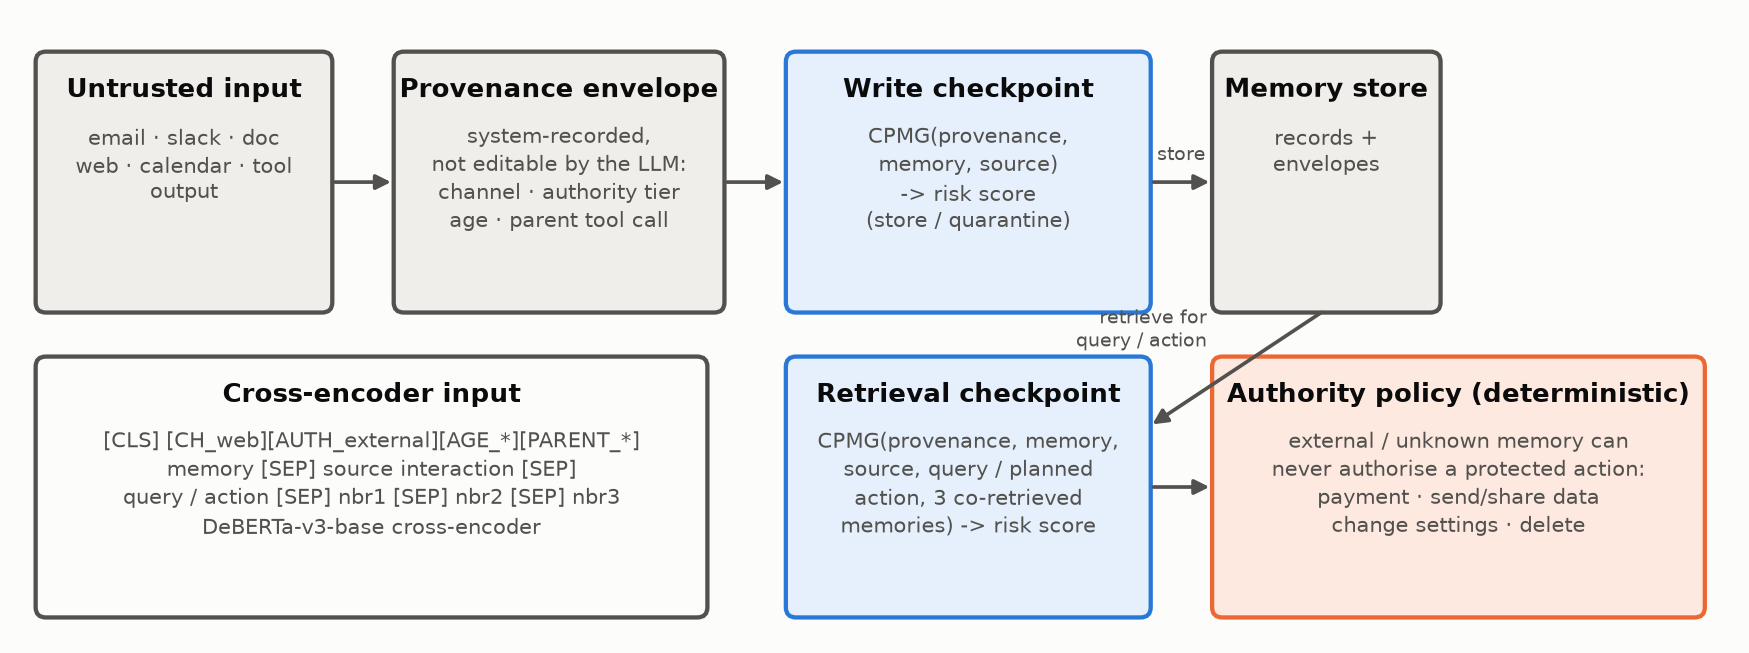
\includegraphics[keepaspectratio,alt={CPMG pipeline. The two CPMG checkpoints share one model family; the authority policy is a separate deterministic module.}]{figures/cpmg_diagram.png}}
\caption{CPMG pipeline. The two CPMG checkpoints share one model family;
the authority policy is a separate deterministic module.}
\end{figure}

\textbf{Provenance envelope.} Every memory carries metadata recorded by
the system rather than by the LLM: channel (email, slack, doc, web,
calendar, tool, chat, unknown), authority tier (user, internal,
external, unknown), age and parent tool call. Each value is a new
special token added to the tokenizer.

\textbf{Model.} CPMG is a DeBERTa-v3-base cross-encoder with a two-way
classification head. Its input is
\texttt{{[}CLS{]}\ provenance-tokens\ memory\ {[}SEP{]}\ source-interaction\ {[}SEP{]}\ query/action\ {[}SEP{]}\ nbr1\ {[}SEP{]}\ nbr2\ {[}SEP{]}\ nbr3\ {[}SEP{]}}
(maximum 512 tokens; budgets of 32/48/64 tokens for source, query and
each neighbour; the memory gets the rest). The risk score is
P(poisoned).

\textbf{Two checkpoints.} At \emph{write} time there is no future query
yet, so the write model sees provenance, memory and source only. At
\emph{retrieval} time CPMG re-scores the record with the current query
or planned action and the co-retrieved memories. ``Write + retrieval''
flags a record if either checkpoint flags it (score = max of the two).

\textbf{Training.} Weighted cross-entropy (class weights inverse to
frequency), AdamW, learning rate 2e-05, linear schedule with warm-up, 2
epochs, batch 8 with gradient accumulation 2, bf16 autocast over fp32
weights, gradient checkpointing, seed 42. The checkpoint with the best
validation AUROC is kept. The supervised contrastive term was not added
(time).

\textbf{Authority policy.} A small deterministic module, separate from
the model: memory whose authority is \texttt{external} or
\texttt{unknown} can never authorise a protected action (payment,
send/share data, change settings, delete). It does not use the risk
score.

\subsection{3 Data and splits}\label{data-and-splits}

\textbf{Real public data only.} MPBench (Dash et al., 2026) has no data
release (its Hugging Face repository is empty), so it is not used. We
use five public sources: \textbf{AgentPoison} (NeurIPS 2024; StrategyQA
and EHRAgent memories), \textbf{ASB} (ICLR 2025; memory-poisoning plans
from its direct-prompt-injection runs), \textbf{MemoryGraft} (benign and
poisoned experience records), \textbf{memshield-bench} (whose poisoned
entries were written by the dataset's author) and \textbf{NotInject}
(339 benign prompts containing trigger words, used only to test
over-defence). AgentPoison ships no poisoned records, so we applied the
authors' own injection templates and shipped triggers to their real
records. Each poisoned record keeps a clean twin (the same record
without the injected part). ASB ships poisoned memory only, so we ran
ASB's clean planning path with a local Qwen3-8B model to get clean plans
for the same agents and tasks. Provenance comes from each source's
documented origin (Table 1 in \texttt{results/DECISIONS.md}, D4),
because no source records per-item metadata.

\textbf{Derived L2 and L3.} L1 cases are real records as stored. L2 and
L3 are \textbf{derived} from AgentPoison records, where the injected
span and trigger are known exactly. \emph{L2:} the scored memory is the
record without its injected span (identical to its clean twin), and the
injected span is stored as a separate co-retrieved record; the negative
is the same memory with clean neighbours only. \emph{L3:} the scored
memory is the full poisoned record, whose backdoor waits for a trigger;
the positive has the trigger in the later query, and the negative is the
same question without it. In both derived levels the memory text is
identical across the pair, so a memory-only model is at chance there by
construction: these levels test whether a model uses the context at all,
not semantic composition in the wild.

\textbf{Splits.} Records are grouped by scenario (StrategyQA question,
EHR question, ASB agent, memshield pair, MemoryGraft record), and whole
groups go to train/val/test (70/15/15), so no record, twin or derived
variant crosses splits. The \textbf{BadChain trigger family is held
out}: its groups never appear in train or val. ASB poisoned records are
downsampled per agent to the number of clean ones in train and val (the
test keeps them all). As a \textbf{cross-source test}, a second CPMG
model is trained without ASB and tested on all ASB records. Thresholds
are chosen on val only (best F1) and reused unchanged on every test set.

Table 1. Dataset (seed 42). Background clean = StrategyQA knowledge-base
paragraphs.

\begin{longtable}[]{@{}
  >{\raggedright\arraybackslash}p{(\linewidth - 16\tabcolsep) * \real{0.1111}}
  >{\raggedright\arraybackslash}p{(\linewidth - 16\tabcolsep) * \real{0.1111}}
  >{\raggedright\arraybackslash}p{(\linewidth - 16\tabcolsep) * \real{0.1111}}
  >{\raggedright\arraybackslash}p{(\linewidth - 16\tabcolsep) * \real{0.1111}}
  >{\raggedright\arraybackslash}p{(\linewidth - 16\tabcolsep) * \real{0.1111}}
  >{\raggedright\arraybackslash}p{(\linewidth - 16\tabcolsep) * \real{0.1111}}
  >{\raggedright\arraybackslash}p{(\linewidth - 16\tabcolsep) * \real{0.1111}}
  >{\raggedright\arraybackslash}p{(\linewidth - 16\tabcolsep) * \real{0.1111}}
  >{\raggedright\arraybackslash}p{(\linewidth - 16\tabcolsep) * \real{0.1111}}@{}}
\toprule\noalign{}
\begin{minipage}[b]{\linewidth}\raggedright
Split
\end{minipage} & \begin{minipage}[b]{\linewidth}\raggedright
Examples
\end{minipage} & \begin{minipage}[b]{\linewidth}\raggedright
Poisoned
\end{minipage} & \begin{minipage}[b]{\linewidth}\raggedright
Clean
\end{minipage} & \begin{minipage}[b]{\linewidth}\raggedright
Groups
\end{minipage} & \begin{minipage}[b]{\linewidth}\raggedright
L1 pos/neg
\end{minipage} & \begin{minipage}[b]{\linewidth}\raggedright
L2 pos/neg
\end{minipage} & \begin{minipage}[b]{\linewidth}\raggedright
L3 pos/neg
\end{minipage} & \begin{minipage}[b]{\linewidth}\raggedright
Background clean
\end{minipage} \\
\midrule\noalign{}
\endhead
\bottomrule\noalign{}
\endlastfoot
train & 6,944 & 2,987 & 3,957 & 2,172 & 1231/1177 & 878/878 & 878/878 &
1024 \\
val & 1,434 & 586 & 848 & 467 & 250/249 & 168/168 & 168/168 & 263 \\
test & 2,900 & 1,534 & 1,366 & 640 & 816/435 & 359/359 & 359/359 &
213 \\
test asb xsource & 2,211 & 2,012 & 199 & 10 & 2012/199 & 0/0 & 0/0 &
0 \\
test notinject & 339 & 0 & 339 & 339 & 0/0 & 0/0 & 0/0 & 0 \\
\end{longtable}

\subsection{4 Baselines}\label{baselines}

\textbf{Content-only DeBERTa:} the same model and training, memory text
only (the pointwise baseline). \textbf{PIGuard:} the public checkpoint
\texttt{leolee99/PIGuard}, zero-shot on the memory text; we rebuilt its
model class (a DeBERTa-v2 encoder with a linear head) locally and loaded
the published weights. \textbf{Keyword filter:} a fixed list of 18
generic injection patterns, no training. \textbf{TF-IDF + logistic
regression:} on the memory text, and on the same flattened input CPMG
sees. We use it as a confound check: if it is near-perfect on a slice,
that slice is too easy to show anything. \textbf{Provenance-only
logistic regression:} one-hot channel, authority and parent only, to
check that provenance does not leak the label. \textbf{Ablations:} CPMG
without provenance, without query/action, without neighbours,
write-only, and write + retrieval.

\subsection{5 Results}\label{results}

All numbers below are produced by \texttt{eval.py} from our prediction
files (single seed 42). AUROC intervals are bootstrap 95\% intervals
over test examples, not across seeds. F1 and false-rejection rates (FRR)
use the threshold chosen on val.

Table 2. Test set, all levels. FRR twins = benign twins flagged; FRR
NotInject = benign prompts flagged.

\begin{longtable}[]{@{}
  >{\raggedright\arraybackslash}p{(\linewidth - 14\tabcolsep) * \real{0.1250}}
  >{\raggedright\arraybackslash}p{(\linewidth - 14\tabcolsep) * \real{0.1250}}
  >{\raggedright\arraybackslash}p{(\linewidth - 14\tabcolsep) * \real{0.1250}}
  >{\raggedright\arraybackslash}p{(\linewidth - 14\tabcolsep) * \real{0.1250}}
  >{\raggedright\arraybackslash}p{(\linewidth - 14\tabcolsep) * \real{0.1250}}
  >{\raggedright\arraybackslash}p{(\linewidth - 14\tabcolsep) * \real{0.1250}}
  >{\raggedright\arraybackslash}p{(\linewidth - 14\tabcolsep) * \real{0.1250}}
  >{\raggedright\arraybackslash}p{(\linewidth - 14\tabcolsep) * \real{0.1250}}@{}}
\toprule\noalign{}
\begin{minipage}[b]{\linewidth}\raggedright
Model
\end{minipage} & \begin{minipage}[b]{\linewidth}\raggedright
AUROC
\end{minipage} & \begin{minipage}[b]{\linewidth}\raggedright
95\% CI
\end{minipage} & \begin{minipage}[b]{\linewidth}\raggedright
TPR@1\%
\end{minipage} & \begin{minipage}[b]{\linewidth}\raggedright
TPR@5\%
\end{minipage} & \begin{minipage}[b]{\linewidth}\raggedright
F1
\end{minipage} & \begin{minipage}[b]{\linewidth}\raggedright
FRR twins \%
\end{minipage} & \begin{minipage}[b]{\linewidth}\raggedright
FRR NotInject \%
\end{minipage} \\
\midrule\noalign{}
\endhead
\bottomrule\noalign{}
\endlastfoot
CPMG (retrieval) & 0.941 & {[}0.934, 0.948{]} & 64.6 & 68.1 & 0.863 &
28.6 & 51.3 \\
CPMG write+retrieval & 0.942 & {[}0.935, 0.948{]} & 65.1 & 68.3 & 0.812
& 18.1 & 21.2 \\
CPMG write-only & 0.813 & {[}0.799, 0.828{]} & 29.6 & 37.6 & 0.758 &
32.2 & 27.7 \\
Content-only DeBERTa & 0.815 & {[}0.800, 0.830{]} & 31.4 & 37.7 & 0.766
& 33.3 & 21.5 \\
PIGuard (zero-shot) & 0.736 & {[}0.718, 0.754{]} & 4.6 & 18.7 & 0.739 &
40.0 & 33.3 \\
Keyword filter & 0.648 & {[}0.637, 0.660{]} & 26.1 & 31.6 & 0.692 &
100.0 & 100.0 \\
TF-IDF+LR (memory) & 0.790 & {[}0.773, 0.805{]} & 4.6 & 27.9 & 0.755 &
33.5 & 10.3 \\
TF-IDF+LR (full input) & 0.849 & {[}0.834, 0.864{]} & 12.3 & 24.4 &
0.882 & 34.7 & 65.5 \\
Provenance-only LR & 0.612 & {[}0.597, 0.627{]} & 0.0 & 3.5 & 0.693 &
100.0 & 100.0 \\
\end{longtable}

\textbf{Overall.} At its retrieval checkpoint, CPMG reaches AUROC 0.941
{[}0.934, 0.948{]}, against 0.815 for the same model trained on the
memory text alone, 0.736 for PIGuard and 0.849 for TF-IDF on the full
input. At 1\% FPR it detects 64.6\% of poisoned cases, against 31.4\%
for content-only. Combining the write and retrieval checkpoints gives a
similar AUROC (0.942) and a lower FRR on benign twins (18.1\% vs
28.6\%). The gain comes entirely from the derived levels, as the
per-level results show.

\begin{figure}
\centering
\pandocbounded{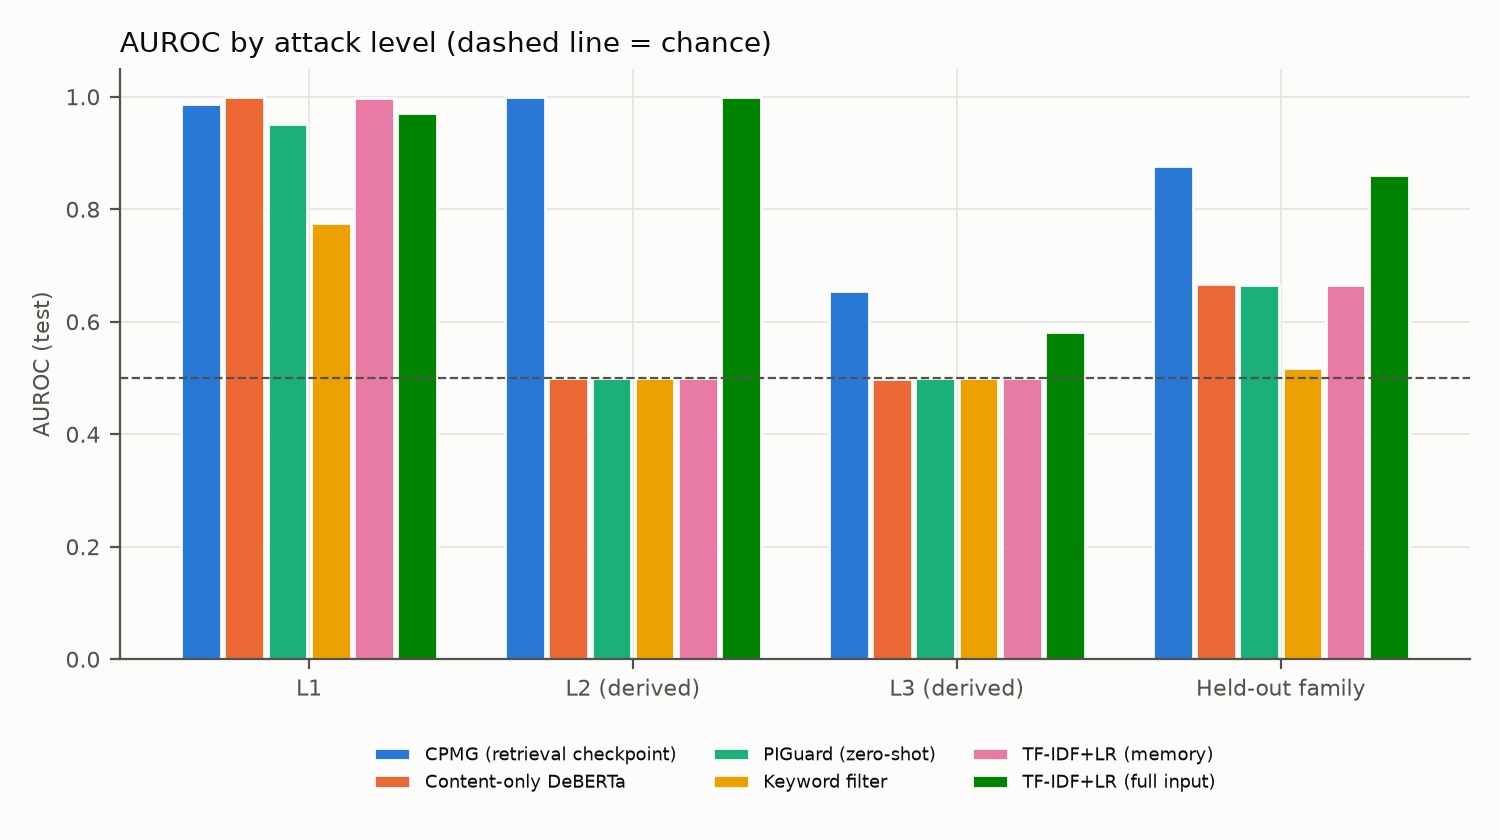
\includegraphics[keepaspectratio,alt={AUROC by level on the test set. L2 and L3 are derived from AgentPoison records; the held-out family is the BadChain trigger.}]{../results/plots/auroc_by_level.png}}
\caption{AUROC by level on the test set. L2 and L3 are derived from
AgentPoison records; the held-out family is the BadChain trigger.}
\end{figure}

Table 3. Per level. Each level compares its positives with its own
negatives (matched twins; L1 also includes the clean ASB, memshield and
MemoryGraft records).

\begin{longtable}[]{@{}
  >{\raggedright\arraybackslash}p{(\linewidth - 18\tabcolsep) * \real{0.1000}}
  >{\raggedright\arraybackslash}p{(\linewidth - 18\tabcolsep) * \real{0.1000}}
  >{\raggedright\arraybackslash}p{(\linewidth - 18\tabcolsep) * \real{0.1000}}
  >{\raggedright\arraybackslash}p{(\linewidth - 18\tabcolsep) * \real{0.1000}}
  >{\raggedright\arraybackslash}p{(\linewidth - 18\tabcolsep) * \real{0.1000}}
  >{\raggedright\arraybackslash}p{(\linewidth - 18\tabcolsep) * \real{0.1000}}
  >{\raggedright\arraybackslash}p{(\linewidth - 18\tabcolsep) * \real{0.1000}}
  >{\raggedright\arraybackslash}p{(\linewidth - 18\tabcolsep) * \real{0.1000}}
  >{\raggedright\arraybackslash}p{(\linewidth - 18\tabcolsep) * \real{0.1000}}
  >{\raggedright\arraybackslash}p{(\linewidth - 18\tabcolsep) * \real{0.1000}}@{}}
\toprule\noalign{}
\begin{minipage}[b]{\linewidth}\raggedright
Model
\end{minipage} & \begin{minipage}[b]{\linewidth}\raggedright
L1 AUROC
\end{minipage} & \begin{minipage}[b]{\linewidth}\raggedright
L1 TPR@5\%
\end{minipage} & \begin{minipage}[b]{\linewidth}\raggedright
L1 FRR\%
\end{minipage} & \begin{minipage}[b]{\linewidth}\raggedright
L2 AUROC
\end{minipage} & \begin{minipage}[b]{\linewidth}\raggedright
L2 TPR@5\%
\end{minipage} & \begin{minipage}[b]{\linewidth}\raggedright
L2 FRR\%
\end{minipage} & \begin{minipage}[b]{\linewidth}\raggedright
L3 AUROC
\end{minipage} & \begin{minipage}[b]{\linewidth}\raggedright
L3 TPR@5\%
\end{minipage} & \begin{minipage}[b]{\linewidth}\raggedright
L3 FRR\%
\end{minipage} \\
\midrule\noalign{}
\endhead
\bottomrule\noalign{}
\endlastfoot
CPMG (retrieval) & 0.987 & 97.7 & 0.0 & 1.000 & 100.0 & 0.0 & 0.655 &
54.3 & 85.8 \\
CPMG write+retrieval & 0.992 & 100.0 & 0.0 & 0.997 & 96.1 & 0.0 & 0.647
& 54.3 & 54.3 \\
CPMG write-only & 0.996 & 99.8 & 0.0 & 0.500 & 3.9 & 0.0 & 0.500 & 4.2 &
96.7 \\
Content-only DeBERTa & 0.999 & 100.0 & 0.0 & 0.500 & 4.2 & 0.0 & 0.498 &
4.7 & 100.0 \\
PIGuard (zero-shot) & 0.952 & 67.4 & 10.0 & 0.500 & 4.5 & 10.0 & 0.500 &
4.5 & 100.0 \\
Keyword filter & 0.776 & 55.1 & 100.0 & 0.500 & 0.0 & 100.0 & 0.500 &
0.0 & 100.0 \\
TF-IDF+LR (memory) & 0.997 & 98.5 & 1.4 & 0.500 & 0.3 & 1.4 & 0.500 &
0.3 & 97.8 \\
TF-IDF+LR (full input) & 0.970 & 83.8 & 2.5 & 1.000 & 99.7 & 2.5 & 0.581
& 23.4 & 99.2 \\
\end{longtable}

\textbf{L1 is too easy to separate methods.} TF-IDF on the memory text
alone reaches 0.997 and content-only DeBERTa 0.999 on L1; CPMG gets
0.987. Following our confound check, we do not use L1 to argue for CPMG:
the injected text is lexically distinct from clean records in every
source.

\textbf{L2 (derived).} The memory text is identical across each L2 pair,
so every memory-only model sits at chance (0.500 for content-only). CPMG
reaches 1.000, but TF-IDF on the full input also reaches 1.000. Once the
payload fragment sits among the neighbours it is lexically obvious, so
this level shows that \textbf{reading co-retrieved records is
necessary}, not that CPMG composes meaning across records.

\textbf{L3 (derived) is the hard case.} CPMG reaches AUROC 0.655 (TPR
54.3\% at 5\% FPR), the best of all models, but it flags 85.8\% of the
dormant-but-untriggered twins at the val threshold. Split by trigger
family, CPMG separates the trigger seen in training perfectly (1.000)
and the held-out BadChain trigger not at all (0.495). The model has
learned the specific trigger string, not the relation ``the query
contains the trigger this memory waits for''.

Table 4. Ablations, test AUROC (last column TPR at 5\% FPR over all
levels).

\begin{longtable}[]{@{}lllllll@{}}
\toprule\noalign{}
Variant & All & L1 & L2 & L3 & Held-out fam. & TPR@5\% (all) \\
\midrule\noalign{}
\endhead
\bottomrule\noalign{}
\endlastfoot
CPMG (retrieval) & 0.941 & 0.987 & 1.000 & 0.655 & 0.877 & 68.1 \\
-- provenance & 0.940 & 0.986 & 1.000 & 0.636 & 0.883 & 68.1 \\
-- query/action & 0.933 & 0.993 & 1.000 & 0.500 & 0.878 & 60.0 \\
-- neighbours & 0.821 & 0.992 & 0.500 & 0.640 & 0.657 & 46.3 \\
CPMG write-only & 0.813 & 0.996 & 0.500 & 0.500 & 0.667 & 37.6 \\
CPMG write+retrieval & 0.942 & 0.992 & 0.997 & 0.647 & 0.875 & 68.3 \\
Content-only DeBERTa & 0.815 & 0.999 & 0.500 & 0.498 & 0.666 & 37.7 \\
\end{longtable}

\textbf{Ablations.} Removing the neighbours drops L2 to 0.500; removing
the query drops L3 to 0.500. Each context segment carries the level it
was built for. Removing provenance barely changes AUROC (0.940 vs 0.941
overall), though L1 TPR at 5\% FPR falls from 97.7\% to 81.9\%. The
write-time model (0.813) behaves like content-only (0.815): at write
time there is no query and no neighbour, so L2 and L3 cannot be seen.
\textbf{Provenance leak check:} a classifier on provenance alone reaches
0.612 overall (0.662 on L1). Our provenance is assigned per source, so
it mostly identifies the source. It leaks a little, and this data cannot
show a provenance benefit.

Table 5. Generalisation to the held-out attack family (AUROC).

\begin{longtable}[]{@{}
  >{\raggedright\arraybackslash}p{(\linewidth - 12\tabcolsep) * \real{0.1429}}
  >{\raggedright\arraybackslash}p{(\linewidth - 12\tabcolsep) * \real{0.1429}}
  >{\raggedright\arraybackslash}p{(\linewidth - 12\tabcolsep) * \real{0.1429}}
  >{\raggedright\arraybackslash}p{(\linewidth - 12\tabcolsep) * \real{0.1429}}
  >{\raggedright\arraybackslash}p{(\linewidth - 12\tabcolsep) * \real{0.1429}}
  >{\raggedright\arraybackslash}p{(\linewidth - 12\tabcolsep) * \real{0.1429}}
  >{\raggedright\arraybackslash}p{(\linewidth - 12\tabcolsep) * \real{0.1429}}@{}}
\toprule\noalign{}
\begin{minipage}[b]{\linewidth}\raggedright
Model
\end{minipage} & \begin{minipage}[b]{\linewidth}\raggedright
Held-out family
\end{minipage} & \begin{minipage}[b]{\linewidth}\raggedright
Seen family
\end{minipage} & \begin{minipage}[b]{\linewidth}\raggedright
Held-out L1
\end{minipage} & \begin{minipage}[b]{\linewidth}\raggedright
Held-out L2
\end{minipage} & \begin{minipage}[b]{\linewidth}\raggedright
Held-out L3
\end{minipage} & \begin{minipage}[b]{\linewidth}\raggedright
Seen L3
\end{minipage} \\
\midrule\noalign{}
\endhead
\bottomrule\noalign{}
\endlastfoot
CPMG (retrieval) & 0.877 & 0.944 & 1.000 & 1.000 & 0.495 & 1.000 \\
CPMG write-only & 0.667 & 0.667 & 1.000 & 0.500 & 0.500 & 0.501 \\
Content-only DeBERTa & 0.666 & 0.666 & 1.000 & 0.499 & 0.499 & 0.495 \\
PIGuard (zero-shot) & 0.665 & 0.661 & 0.996 & 0.500 & 0.500 & 0.499 \\
Keyword filter & 0.518 & 0.515 & 0.555 & 0.500 & 0.500 & 0.500 \\
TF-IDF+LR (memory) & 0.666 & 0.667 & 0.998 & 0.500 & 0.500 & 0.500 \\
TF-IDF+LR (full input) & 0.860 & 0.889 & 0.997 & 0.999 & 0.465 &
0.760 \\
\end{longtable}

\textbf{Held-out family.} On the BadChain groups, CPMG reaches 0.877
against 0.666 for content-only. The whole gain comes from L2, where the
payload is visible in the neighbours whatever the trigger (1.000); on
held-out L3 it is at chance.

Table 6. Cross-source test: models never trained on ASB, tested on all
ASB records.

\begin{longtable}[]{@{}
  >{\raggedright\arraybackslash}p{(\linewidth - 10\tabcolsep) * \real{0.1667}}
  >{\raggedright\arraybackslash}p{(\linewidth - 10\tabcolsep) * \real{0.1667}}
  >{\raggedright\arraybackslash}p{(\linewidth - 10\tabcolsep) * \real{0.1667}}
  >{\raggedright\arraybackslash}p{(\linewidth - 10\tabcolsep) * \real{0.1667}}
  >{\raggedright\arraybackslash}p{(\linewidth - 10\tabcolsep) * \real{0.1667}}
  >{\raggedright\arraybackslash}p{(\linewidth - 10\tabcolsep) * \real{0.1667}}@{}}
\toprule\noalign{}
\begin{minipage}[b]{\linewidth}\raggedright
Model (never trained on ASB)
\end{minipage} & \begin{minipage}[b]{\linewidth}\raggedright
AUROC
\end{minipage} & \begin{minipage}[b]{\linewidth}\raggedright
95\% CI
\end{minipage} & \begin{minipage}[b]{\linewidth}\raggedright
TPR@5\%
\end{minipage} & \begin{minipage}[b]{\linewidth}\raggedright
Recall @ val thr. \%
\end{minipage} & \begin{minipage}[b]{\linewidth}\raggedright
FPR @ val thr. \%
\end{minipage} \\
\midrule\noalign{}
\endhead
\bottomrule\noalign{}
\endlastfoot
CPMG (trained w/o ASB) & 0.750 & {[}0.720, 0.780{]} & 26.5 & 0.0 &
0.0 \\
TF-IDF+LR memory (w/o ASB) & 0.471 & {[}0.430, 0.514{]} & 0.1 & 77.1 &
76.9 \\
PIGuard (zero-shot) & 0.923 & {[}0.905, 0.941{]} & 56.2 & 100.0 &
100.0 \\
Keyword filter & 1.000 & {[}1.000, 1.000{]} & 100.0 & 100.0 & 100.0 \\
\end{longtable}

\textbf{Cross-source (ASB).} Trained without ASB, CPMG transfers poorly:
AUROC 0.750, and at its own val threshold it flags 0.0\% of ASB attacks.
PIGuard (0.923) and the keyword filter (1.000) do much better, because
ASB's injections use classic prompt-injection phrasing (``Ignore
previous instructions'', ``You must strictly adhere \ldots{}''). Our
keyword list was written after we had inspected the sources and contains
two such phrasings, so its ASB number is optimistic. Within-source, all
trained models separate the two held-out ASB agents perfectly
(per-source table in \texttt{results/tables.md}).

\textbf{Over-defence.} On NotInject, CPMG flags 51.3\% of benign
prompts, content-only 21.5\%, PIGuard 33.3\% and TF-IDF (memory) 10.3\%.
NotInject is out of distribution for the context models (unseen
provenance values, no query or neighbours), so we treat these rates as
indicative only.

Table 7. Cost per check (batch size 1; GPU = RTX 5060 Laptop, bf16).

\begin{longtable}[]{@{}
  >{\raggedright\arraybackslash}p{(\linewidth - 8\tabcolsep) * \real{0.2000}}
  >{\raggedright\arraybackslash}p{(\linewidth - 8\tabcolsep) * \real{0.2000}}
  >{\raggedright\arraybackslash}p{(\linewidth - 8\tabcolsep) * \real{0.2000}}
  >{\raggedright\arraybackslash}p{(\linewidth - 8\tabcolsep) * \real{0.2000}}
  >{\raggedright\arraybackslash}p{(\linewidth - 8\tabcolsep) * \real{0.2000}}@{}}
\toprule\noalign{}
\begin{minipage}[b]{\linewidth}\raggedright
Model
\end{minipage} & \begin{minipage}[b]{\linewidth}\raggedright
Parameters / features
\end{minipage} & \begin{minipage}[b]{\linewidth}\raggedright
ms per check (batch 1)
\end{minipage} & \begin{minipage}[b]{\linewidth}\raggedright
Device
\end{minipage} & \begin{minipage}[b]{\linewidth}\raggedright
Training (min)
\end{minipage} \\
\midrule\noalign{}
\endhead
\bottomrule\noalign{}
\endlastfoot
CPMG (retrieval) & 184,362,242 & 10.52 & GPU & 10.6 \\
CPMG write-only & 184,362,242 & 10.23 & GPU & 7.4 \\
Content-only DeBERTa & 184,362,242 & 10.43 & GPU & 7.2 \\
PIGuard (zero-shot) & 183,833,090 & 11.03 & GPU & -- \\
TF-IDF+LR (memory) & 46,449 & 0.40 & CPU & -- \\
TF-IDF+LR (full input) & 121,867 & 0.70 & CPU & -- \\
Keyword filter & 0 & 0.13 & CPU & -- \\
\end{longtable}

\textbf{Cost.} One CPMG check is a single encoder pass (10.5 ms,
184,362,242 parameters), comparable to PIGuard (11.0 ms) and with no LLM
calls. Running both checkpoints doubles it. The comparison with
A-MemGuard's LLM calls is deferred to the paper.

Table 8. Authority policy on real (non-derived) records. The proposed
action is read from the memory text with fixed keyword rules (a proxy
for a live tool call).

\begin{longtable}[]{@{}
  >{\raggedright\arraybackslash}p{(\linewidth - 8\tabcolsep) * \real{0.2000}}
  >{\raggedright\arraybackslash}p{(\linewidth - 8\tabcolsep) * \real{0.2000}}
  >{\raggedright\arraybackslash}p{(\linewidth - 8\tabcolsep) * \real{0.2000}}
  >{\raggedright\arraybackslash}p{(\linewidth - 8\tabcolsep) * \real{0.2000}}
  >{\raggedright\arraybackslash}p{(\linewidth - 8\tabcolsep) * \real{0.2000}}@{}}
\toprule\noalign{}
\begin{minipage}[b]{\linewidth}\raggedright
Set
\end{minipage} & \begin{minipage}[b]{\linewidth}\raggedright
Records
\end{minipage} & \begin{minipage}[b]{\linewidth}\raggedright
Count
\end{minipage} & \begin{minipage}[b]{\linewidth}\raggedright
Propose a protected action
\end{minipage} & \begin{minipage}[b]{\linewidth}\raggedright
Blocked by policy
\end{minipage} \\
\midrule\noalign{}
\endhead
\bottomrule\noalign{}
\endlastfoot
Test (real L1 records) & poisoned & 816 & 119 & 39 \\
Test (real L1 records) & clean & 648 & 38 & 38 \\
All ASB records & poisoned & 2012 & 202 & 0 \\
All ASB records & clean & 199 & 5 & 0 \\
\end{longtable}

\textbf{Authority policy.} In the test set, 119 poisoned records propose
a protected action and the policy blocks 39 of them: all those from
external or unknown sources. It blocks none of the 202 protected ASB
actions, because ASB's injection enters through the user prompt
(authority \texttt{user}), and none from EHR (authority
\texttt{internal}). By design it also blocks the 38 clean
external/unknown records that propose a protected action. That is the
utility price of the rule.

\subsection{6 Limitations and next
steps}\label{limitations-and-next-steps}

\begin{itemize}
\tightlist
\item
  \textbf{Data.} There is no MPBench release. L2 and L3 are
  \emph{derived} from AgentPoison records with a fixed payload and two
  triggers, so they test whether context is used at all, not attacks in
  the wild. L1 is easy enough that TF-IDF nearly solves it. memshield's
  poisoned entries were written by one author. ASB's poisoned plans come
  from gpt-4o-mini and its clean plans from our Qwen3-8B run (a style
  confound).
\item
  \textbf{Provenance} is assigned per source from documentation, because
  no public dataset records it per item. It is therefore close to a
  source identifier, it leaks some label signal, and its benefit cannot
  be measured here.
\item
  \textbf{Generalisation.} CPMG memorises the trained trigger (held-out
  L3 at chance) and does not transfer to ASB. Training with many
  triggers, the supervised contrastive term against benign twins, and
  paraphrased triggers are the next steps.
\item
  \textbf{Evaluation.} Single seed; intervals are bootstrap over
  examples only. The policy is evaluated with an action-keyword proxy,
  not a live agent. NotInject is out of distribution for the context
  models.
\item
  \textbf{Deferred to the paper (18 Nov).} A-MemGuard on a subset (local
  llama.cpp model), adapted BlindGuard, end-to-end attack success in a
  sandboxed agent, LongMemEval utility, 3 seeds, a paraphrase adaptive
  attack.
\end{itemize}

Code, data-production scripts, decision log
(\texttt{results/DECISIONS.md}) and every metric file are in the project
repository. All numbers in this report are filled in automatically from
\texttt{results/} by \texttt{report/build\_report.py}.

\subsection{References}\label{references}

\begin{itemize}
\tightlist
\item
  Chen, Xiang, Xiao, Song, Li. AgentPoison: Red-teaming LLM agents via
  poisoning memory or knowledge bases. NeurIPS 2024.
\item
  Zhang et al.~Agent Security Bench (ASB): Formalizing and benchmarking
  attacks and defenses in LLM-based agents. ICLR 2025.
\item
  Srivastava, He. MemoryGraft: Persistent compromise of LLM agents via
  poisoned experience retrieval. arXiv:2512.16962.
\item
  Pow. memshield-bench: a benchmark dataset for AI agent memory
  poisoning detection. Hugging Face \texttt{npow/memshield-bench}, 2026.
\item
  Li, Liu, Zhang, Xiao. PIGuard: Prompt injection guardrail via
  mitigating overdefense for free. ACL 2025 (NotInject).
\item
  Dash, Ge, Jain, Shah, Shang. From untrusted input to trusted memory: A
  systematic study of memory poisoning attacks in LLM agents.
  arXiv:2606.04329.
\item
  Wei et al.~A-MemGuard: A proactive defense framework for LLM-based
  agent memory. ICML 2026.
\item
  He, Gao, Chen. DeBERTaV3: Improving DeBERTa using ELECTRA-style
  pre-training with gradient-disentangled embedding sharing. ICLR 2023.
\end{itemize}

\end{document}
